%chktex-file 44

Στο παρόν κεφάλαιο, θα πραγματοποιηθεί μια αναλυτική περιγραφή όλων των σταδίων της φάσης ανάπτυξης (development phase) της εφαρμογής. Παράλληλα, θα εξηγήσουμε όλες τις λειτουργίες της εφαμρογής μαζί με τη λογική αυτών, παρουσίαζοντας τμήματα του κώδικα που αναπτύχθηκε.
Ολόκληρος ο κώδικας της εργασίας βρίσκεται στο \hyperref[ch:appendixA]{Παράρτημα Α'} μαζί με σχόλια σχετικά με τη λειτουργία κάθε μεθόδου.

\subsection{Προετοιμασία και Εγκατάσταση}\label{subsec:developSetup}
% H κύρια γλώσσα προγραμματισμού, που συνιστά η Microsoft για την ανάπτυξη εφαρμογών για το headset HoloLens 2 είναι η C\#. H Microsoft, για την συγγραγή κώδικα σε αυτή τη γλώσσα, συνιστά τη χρήση του IDE Visual Studio, ενώ για την εκτέλεση αυτού, τη μηχανή γραφικών Unity.

Αρχικά εγκαταστήσαμε όλα τα απαραίτητα εργαλεία, τα όποια συνιστά η Microsoft για την ανάπτυξη εφαρμογών για το headset HoloLens 2. Αφού η συνιστώμενη γλώσσα προγραμματισμού, την όποια και επιλέξαμε, είναι η C\#, έπρεπε να εγκαταστήσουμε το IDE Visual Studio, τη μηχανή γραφικών Unity, καθώς και το εργαλείο Mixed Reality Feature Tool (\hyperref[fig:mrft]{\schema~\ref*{fig:mrft}}) για την προσθήκη του MRTK στο project.

\begin{figure}[!h]
    \centering
    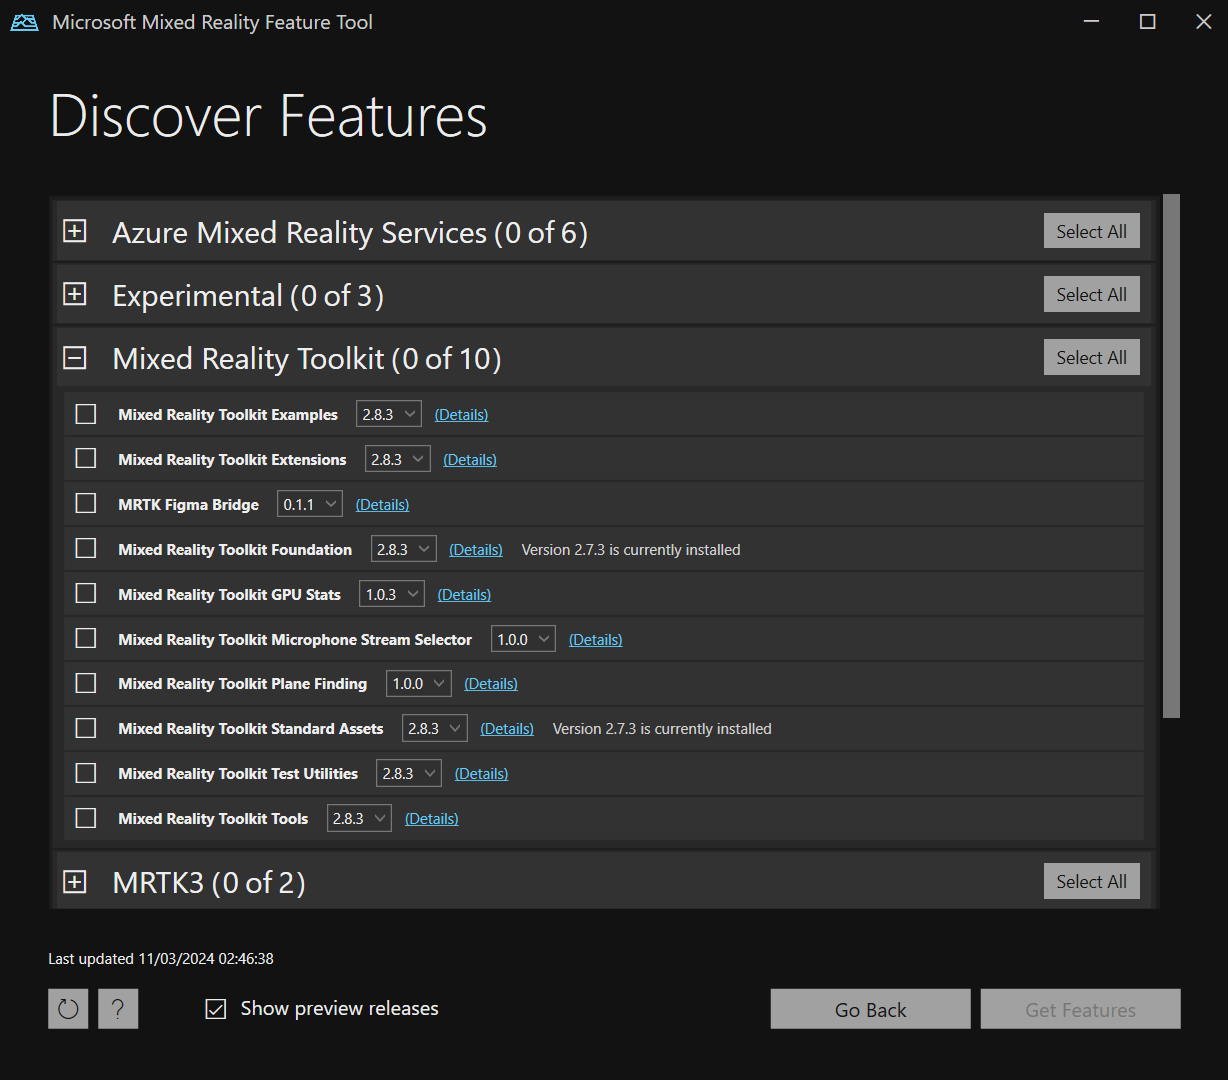
\includegraphics[width=0.8\textwidth]{images/mixed_reality_feature_tool.png}
    \caption{Το Mixed Reality Feature Tool}\label{fig:mrft}
\end{figure}

Όπως αναφέρθηκε και στο προηγούμενο κεφάλαιο (\hyperref[sec:appDesignAndLimitations]{Κεφάλαιο~\ref*{sec:appDesignAndLimitations}}), ένα σημαντικό πρόβλημα, που δημιούργησε το δύσχρηστο documentation, ήταν η έλλειψη καθοδήγησης όσoν αφορά τη συμβατότητα των διάφορων εκδόσεων των προγραμμάτων. Για το λόγο αυτό, δεν επιλέχθηκαν οι πιο πρόσφατες εκδόσεις, αλλά εκδόσεις, οι οποίες χρησιμοποιούνταν κατά κόρον στους διάφορους διαθέσιμους οδηγούς. Ειδικότερα, επιλέχθηκε η Unity 2020.3.48f1 και εγκαταστήθηκε το Visual Studio Community 2019 μαζί με τα απαραίτητα components για την ανάπτυξη εφαρμογών μικτής πραγματικότητας, καθώς και την τελευταία έκδοση του Mixed Reality Feature Tool (version 1.0.2209.0). Επίσης, για τη διαχείριση των εκδόσεων του κώδικα, που αναπτύξαμε, χρησιμοποιήθηκε το λογισμικό Git, ενώ, για την αποθήκευση αυτού, έγινε χρήση της πλατφόρμας GitHub.

Μετά την ολοκλήρωση της εγκατάστασης, πρώτο βήμα στην ανάπτυξη της εφαρμογής ήταν η δημιουργία ενός project στη Unity, το οποίο διαθέτει μια σκηνή με τα αρχικώς απαραίτητα \code{GameObjects}, όπως είναι η Camera, ενώ παρέχει πληθώρα από \code{Components} και Assets. Ωστόσο, αυτές οι `πρώτες ύλες' δεν επαρκούν για την ανάπτυξη εφαρμογών μικτής πραγματικότητας. Για το λόγο αυτό, θα αξιοποιήσουμε το Mixed Reality Feature Tool για την προσθήκη των αναγκαίων packages, όπως αυτά αναφέρονται στον \hyperref[table:mrft]{Πίνακα~\ref*{table:mrft}}, με σημαντκότερο από όλα το MRTK\@.

\begin{table}[!ht]
    \begin{tabularx}{\textwidth}{|X|X|}
        \hline
        Mixed Reality Toolkit Foundation & version 2.7.3 \\
        \hline
        Mixed Reality Toolkit Standard Assets & version 2.7.3 \\
        \hline
        Mixed Reality OpenXR Plugin & version 1.4.0 \\
        \hline
        Microsoft Spatializer & version 2.0.37 \\
        \hline
    \end{tabularx}
    \caption{Packages που ενσωματώθηκαν στο project με τη χρήση του Mixed Reality Feature Tool}\label{table:mrft}
\end{table}

Με την ενσωμάτωση του MRTK, προστίθενται στη σκηνή ορισμένα βασικά \code{GameObjects}, ενώ στο project συμπεριλαμβάνονται απαραίτητα components για την βελτίωση της συμπεριφοράς των εικονικών αντικειμένων και την καλύτερη αλληλεπίδραση του χρήστη με αυτά, assets για τη διαμόρφωση του UI (User Interface) της εφαρμογής, καθώς και λειτουργίες, οι οποίες θα διευκολύνουν σημαντικά την αναπτύξη και δοκιμή της εφαρμογής μας~\cite{polarkev_2022_mrtk2unity}.

Πλέον, η ιεραρχία των \code{GameObjects} στη σκηνή διαμορφώνεται με τον τρόπο που φαίνεται στο \hyperref[fig:developHierarchyMRTK]{\schema~\ref*{fig:developHierarchyMRTK}}.

\begin{figure}[!h]
    \centering
    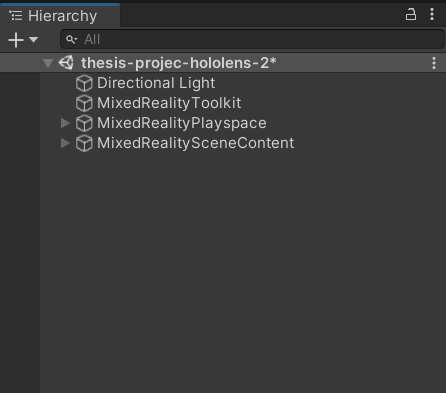
\includegraphics[width=0.8\textwidth]{images/develop_hierarchyAfterMRTK.png}
    \caption{Το hierarchy window μετά την προσθήκη του MRTK}\label{fig:developHierarchyMRTK}
\end{figure}

Τα νέα \code{GameObjects}, που προστέθηκαν, είναι:
\begin{itemize}
    \item \textbf{MixedRealityToolkit}: Αποτελεί το κύριο \code{GameObject} της εργαλειοθήκης, καθώς διαθέτει όλες τις ρυθμίσεις της, όπως για το σύστημα εισόδου (Input System), την κάμερα, την χωρική χαρτογράφηση και άλλα.
    \item \textbf{MixedRealityPlayspace}: Είναι το \code{GameObject} που αντιπροσωπεύει το headset στη σκηνή. Εντός αυτού του αντικειμένου, υπάρχει και το αντικείμενο της κάμερας.
    \item \textbf{MixedRealitySceneContent}: Αποτελεί τον χωρό των εικονικών αντικειμένων. Τα αντικειμένα τοποθετούνται εντός αυτού\\
    τους \code{GameObject}, με σκοπό να εξασφαλιστεί η σωστή κλίμακα αυτών, όταν προβάλλονται στον πραγματικό χώρο.
\end{itemize}

Επιπλέον, το MRTK μας δίνει τη δυνατότητα να κάνουμε προσομοίωση χρήσης της εφαρμογής μέσα από τον Editor της Unity, το οποίο ήταν καθοριστικό στα πρώτα στάδια ανάπτυξης της εφαρμογής για τo debugging και τις δοκιμές αυτής. Τέλος, η λειτουργία Holographic Remoting του MRTK επιτρέπει στη Unity να συνδεθεί με το HoloLens 2 μέσω του Holographic Remoting Player (\hyperref[fig:developHolographicRemotingPlayer]{\schema~\ref*{fig:developHolographicRemotingPlayer}}), ώστε το headset να `τρέξει' την εφαρμογή μας και να δοκιμαστεί υπό πραγματικές συνθήκες~\cite{florianbagarmicrosoft_2023_holographic}. Η λειτουργία αυτή αξιοποιήθηκε στα τελευταία στάδια ανάπτυξης, με σκοπό να ελεγχθεί ταχύτατα η λειτουργικότητα της εφαρμογής, αλλά και για να γίνουν οι απαραίτητες αλλαγές σε προβλήματα που δεν θα μπορούσαμε να εντοπίσουμε κατά την προσομοίωση.

\begin{figure}[!h]
    \centering
    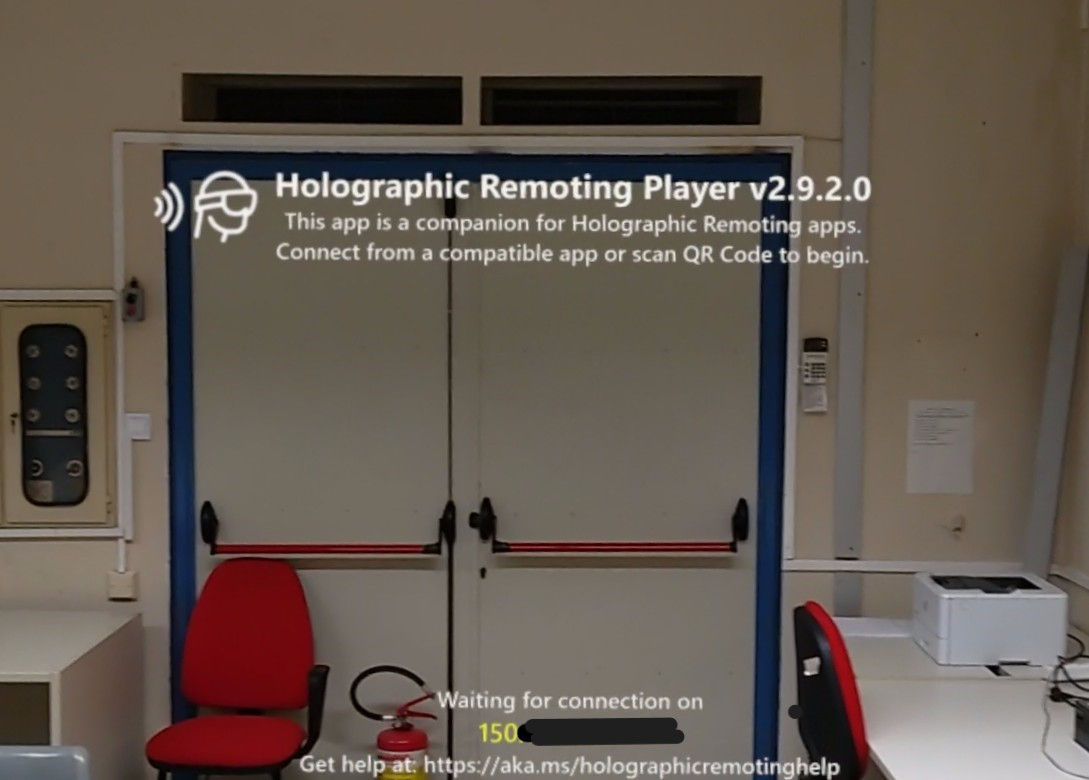
\includegraphics[width=0.8\textwidth]{images/develop_holographicRemotingPlayer.jpg}
    \caption{Το Holographic Remoting Player σε αναμονή σύνδεσης}\label{fig:developHolographicRemotingPlayer}
\end{figure}

\subsection{Οργάνωση του Project}\label{subsec:developOrganization}
Σε αυτή το κεφάλαιο, θα πραγματοποιήσουμε μια μικρή περιήγηση στη σκηνή της εφαρμογής μας. Θα παρουσιάσουμε τα \code{GameObjects} που δημιουργήθηκαν κατά την ανάπτυξη, τον τροπό οργάνωσης αυτών και των \code{Components}, τα οποία συντάξαμε και θα περιγράψουμε συνοπτικά τη λειτουργία τους. Μια αναλύτική περιγραφή όλων των παραπάνων θα δοθεί στα ακόλουθα κεφάλαια.

\begin{figure}[!hb]
    \centering
    \begin{subfigure}{0.5\textwidth}
        \centering
        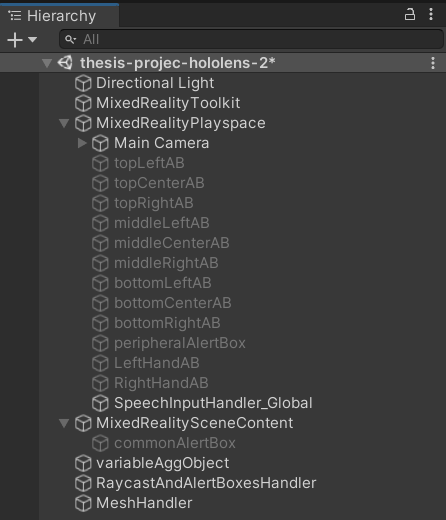
\includegraphics[width=0.9\linewidth]{images/develop_hierarchyFinalOne.png}
        \caption{}\label{fig:developFinalHierarchyWindowOne}
    \end{subfigure}%
    \begin{subfigure}{0.5\textwidth}
        \centering
        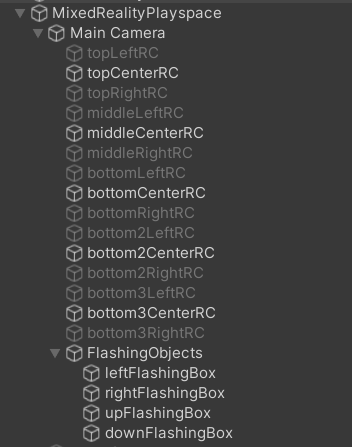
\includegraphics[width=0.825\linewidth]{images/develop_hierarchyFinalTwo.png}
        \caption{}\label{fig:developFinalHierarchyWindowTwo}
    \end{subfigure}%
    \caption{Η τελική μορφή του Hierarchy Window}\label{fig:developFinalHierarchyWindow}
\end{figure}

Αρχικά, οι φάκελοι του project έχουν την ακόλουθη δομή:
\\
\dirtree{%
.1 Thesis-project-2.
.2 Assets.
.3 Audio Files.
.4 \ldots.
.3 Materials.
.4 \ldots.
.3 Scripts.
.4 \_InspectorExtensions.
.5 \ldots.
.4 castModes.
.5 \ldots.
.4 initiators.
.5 \ldots.
.4 \ldots.
.3 \textit{SpatialMapping.obj}.
.3 \textit{SpatialAudio.mixer}.
.3 \ldots.
}

Ειδικότερα, στο φάκελο \textbf{Audio Files}, τοποθετήθηκαν αρχεία ήχου σε μορφή \textbf{.mp3}, ενώ στο φάκελο \textbf{Materials}, τοποθετήθηκαν τα υλικά, τα οποία εφαρμόστηκαν στα GameObjects που δημιοργήσαμε και τους προσδίδουν υφή και χρώμα. Ο φάκελος \textbf{Scripts}, καθώς και οι υποφακέλοι αυτού, περιέχουν αρχεία κώδικα σε μορφή \textbf{.cs} και αποτελούν ουσιαστικά τα \code{Components} που αναπτύξαμε για τα \code{GameObjects} μας, αλλά και μερικά αρχεία για την καλύτερη απεικόνιση πληροφοριών στο Inspector window. Τέλος, εντός του φακέλου \textbf{Assets} υπάρχει το αρχείο SpatialMapping, το οποίο είναι ένα 3D μοντέλο κλειστού χώρου, που χρησιμοποιήθηκε στις προσομοιώσεις και ένα mixer για τον έλεγχο του ήχου.

Σχετικά με τα \code{GameObjects} και τη θέση αυτών (\hyperref[fig:developFinalHierarchyWindow]{\schema~\ref*{fig:developFinalHierarchyWindow}}), παρατηρούμε ότι ορισμένα από αυτά είναι `εμφωλευμένα', εντός των \code{GameObjects} \textbf{MixedRealityPlayspace} και \textbf{MixedRealitySceneContent}. Αυτά αποτελούν τα εικονικά αντικείμενα, τα οποία θα τοποθετούνται και απεικονίζονται στο πραγματικό χώρο. Το ίδιο συμβαίνει και με τα \code{GameObjects}, τα οποία είναι `children' (`παιδιά') της \textbf{Main Camera} με μόνη διαφορά ότι η θέση τους μεταβάλλεται σύνεχως σύμφωνα με την κίνηση του headset, δηλαδή την κίνηση του κεφαλιού του χρήστη. Τα \code{GameObjects}, που δεν βρίσκονται εντός των ειδικά διαμορφωμένων \code{GameObjects} από το MRTK, επιτελούν βοηθητικό ρόλο, καθώς ενσωματώνουν scripts που βοηθούν στη διαχείριση των λειτουργιών της εφαρμογής και των λοιπών \code{GameObjects} στη σκηνή.

Όσον αφορά την ονοματοδοσία των \code{GameObjects}, αυτή καθορίζεται από το σκοπό τους. Συγκεριμένα, αντικείμενα, τα οποία χρησιμοποιούνται για την αναπαραγωγή προειδοποιητικών ήχων, περιέχουν τα γράμματα `AB' στο τέλος του ονόματος, ενώ στην αρχή αυτού αναφέρεται η θέση των αντικειμένων αυτών κατά την έναρξη εκτέλεσης της εφαρμογής, σε CamelCase μορφή. Κάτι αντίστοιχο ισχύει και στην περίπτωση των \code{GameObjects}, τα οποία ενσωματώνουν components για τον εντοπισμό εμποδίων στη διαδρομή του χρήστη. Για την διαφοροποίηση των αντικειμένων αυτών, η κατάληξη της ονομασίας τους είναι `RC'. Αντικκείμενα, τα οποία επιτελούν βοηθητικό ρόλο, όπως αναφέρθηκε και προηγουμένως, διαθέτουν την λέξη `Handler' στην ονομασία τους (από εδώ και στο εξής τα αντικείμενα αυτά μαζί με τα components τους θα αποκαλούνται `handlers').

Τέλος, ειδική αναφορά πρέπει να πραγματοποιηθεί στο \code{GameObject} \textbf{variableAggObject}, στο όποιο έχει προστεθεί το component\\
\hyperref[lst:variablesAggregator]{\textit{\textbf{variablesAggregator.cs}}} (\textit{Assets/Scripts}). Σκοπός του αρχείου είναι να συγκεντρώνει την πλειοψηφία των κοινών μεταβλητών που χρειάζονται περισσότερα του ενός scripts, ορίζοντας αυτές ως public, δηλαδή να είναι προσβάσιμες από άλλες κλάσεις πέρα αυτής στην οποία ορίστηκαν. Με τον τρόπο αυτό, είναι ευκολότερο για εμάς να διαχειριστούμε ένα μεγάλο αριθμό μεταβλητών, τις οποίες συχνά καλούμαστε να αλλάξουμε πριν ή κατά την εκτέλεση της εφαρμογής για λόγους δοκιμής ή διορθώσεων.

\begin{figure}[!h]
    \centering
    \begin{subfigure}{0.5\textwidth}
        \centering
        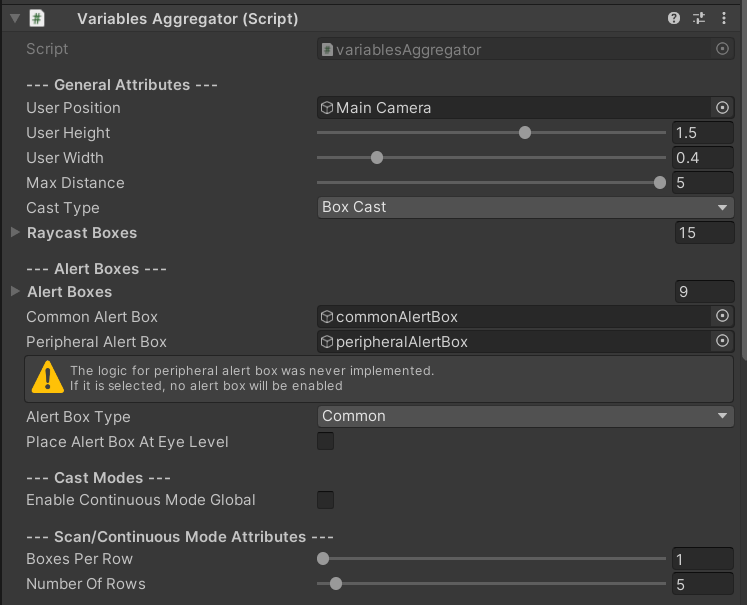
\includegraphics[width=0.9\linewidth]{images/develop_inspVariableAggObjectOne.png}
        \caption{}
    \end{subfigure}%
    \begin{subfigure}{0.5\textwidth}
        \centering
        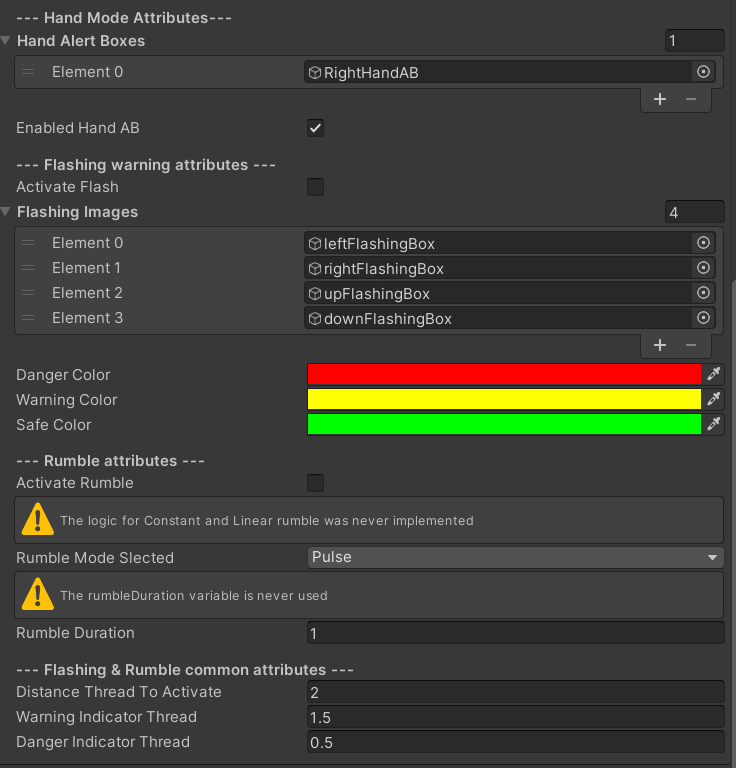
\includegraphics[width=0.9\linewidth]{images/develop_inspVariableAggObjectTwo.png}
        \caption{}
    \end{subfigure}%
    \caption{Το Inspector window για το variableAggObject}\label{fig:developInspVariableAggObject}
\end{figure}

\subsection{Εντοπισμός Εμποδίων}\label{subsec:developObstacleDetection}

Η σημαντικότερη λειτουργία της εφαρμογής αποτελεί ο εντοπισμός των εμποδίων στη διαδρομή ενός χρήστη. Ο χρήστης μπορεί να περιηγηθεί σε ένα κλειστό χώρο, γνωστό ή άγνωστο προς αυτόν. Η εφαρμογεί οφείλει να καταγράψει το χώρο και να αναζητήσει προς την κατεύθυνση πορείας του χρήστη πιθανά εμπόδια. Σε περίπτωση που εντοπίσει κάποιο εμπόδιο, πρέπει να προειδοποιήσει το χρήστη με διάφορους τρόπους (\hyperref[subsec:developWarning]{Κεφάλαιο~\ref*{subsec:developWarning}}), ώστε αυτός, αναλογά με τη θέση και την απόσταση του εμποδίου, να επιλέξει αν επιθυμεί να αλλάξει πορεία κατεύθυνσης ή να προσπεράσει το εμπόδιο.

Για να επιτευχθεί αυτή η λειτουργία, αρχικά, θα πρέπει να πραγματοποιηθεί μια καταγραφεί ο περιβάλλων χώρος του χρήστη. Για αυτό θα αξιοποιήσουμε την τεχνολογία της χωρικής χαρτογράφησης (spatial mapping) που προσφέρει το headset. Ειδικότερα, καθώς η συγκεκριμένη λειτουργία είναι ενργοποιημένοι, ο χρήστης περιστρέφει το κεφάλι του μαζί με το headset προς διάφορες κατευθύνσεις. Με τον τρόπο συλλέγονται πλήθος σημείων, δημιουργόντας ένα νέφος (point cloud) και με βάση τα σημεία αυτά δημιουργείται ένα σύνολο τριγώνων, που αποτελούν το mesh. Διάφοροι παράμετροι σχετικά με τον τρόπο λειτουργίας της χαρτογράφησης μπορούν να τροποποιηθούν.

Η ενεργοποίηση της χωρικής χαρτογράφησης γίνεται μέσα από τις ρυθμίσεις που διαθέτει το \code{GameObject} \textbf{MixedRealityToolkit}, στην καρτέλα `Spatial Awareness' (\hyperref[fig:developMRTKSpatialAwareness]{\schema~\ref*{fig:developMRTKSpatialAwareness}}). Αφού ενεργοποιήσουμε τη λειτουργία και δημιουργήσουμε τα custom profiles μας για την αποθήκευση των τροποποιήσεών μας, πρέπει να δημιουργήσουμε ένα `Spatial Surface Observer', το οποίο αποτελεί ουσιαστικά το αντικείμενο που διαχειρίζεται τον τρόπο δημιουργίας και απεικόνισης των meshes~\cite{mattzmsft_2023_spatial}. Στην δική μας περίπτωση, χρησιμοποιήσαμε δύο Observers, ένας ο οποίος χρησιμοποιήθηκε κάτα την προσομοίωση της εφαρμογής (Spatial Object Mesh Observer~\cite{davidklinems_2022_spatial}) και ένας ο οποίος χρησιμοποιήθηκε κατά τις δοκιμές της εφαρμογής με χρήση του headset (OpenXR Spatial Mesh Observer). Ωστόσο η πλειονότητα των αλλαγών, που πραγματοποιήθηκαν στο setup αυτών, ήταν ίδιες και στις δύο περιπτώσεις.

\begin{figure}[!h]
    \centering
    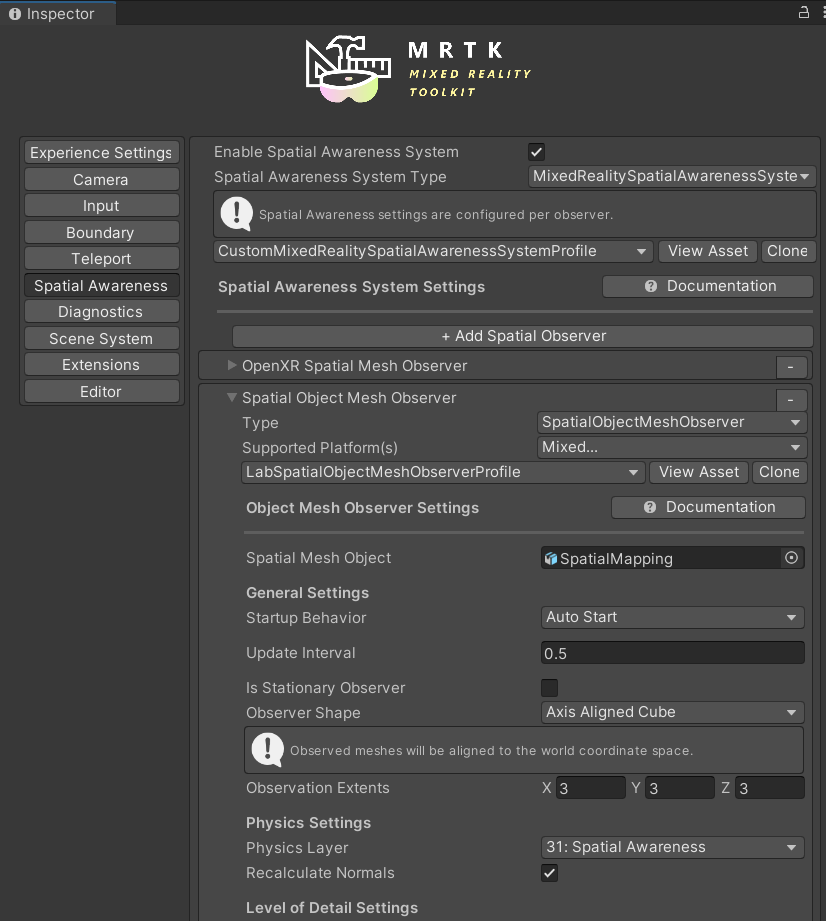
\includegraphics[width=0.6\textwidth]{images/develop_inspMRTKSpatialAwareness.png}
    \caption{Οι ρυθμίσεις της λειτουργίας `Spatial Awareness' και των `Spatial Surface Observers'}\label{fig:developMRTKSpatialAwareness}
\end{figure}

Θα περιγράψουμε περιληπτικά τις κύριες παραμέτρους που αλλάξαμε, καθώς και τις τιμές που θέσαμε~\cite{davidklinems_2022_configuring}:

\begin{itemize}
    \item \textbf{Startup Behavior}: Καθορίζει αν η καταγραφή του χώρου θα ξεκινήσει αμέσως μετά την αρχικοποίηση της λειτουργίας ή αν θα καθοριστεί από τον προγραμματιστή. Θέσαμε την τιμή \textbf{Auto Start}, ώστε η καταγραφεί να αρχίσει με την έναρξη χρήσης της εφαρμογής.
    \item \textbf{Update Interval}: Είναι ο ρυθμός ανανέωσης σε δευτερόλεπτατων δεδομένων του mesh. Για την προσομοίωση, επιλέξαμε το mesh να ανανεώνεται κάθε \textbf{0.5} δευτερόλεπτα, ενώ στις πραγματικές δοκιμές κάθε \textbf{0.1}, αφού οι αλλαγές στο χώρο είναι πιο συχνές.
    \item \textbf{Is Stationary Observer}: Καθορίζει αν ο Observer, που πραγματοποιεί την καταγραφή, θα βρίσκεται σταθερά στο χώρο ή θα κινείται μαζί με τον χρήστη. Επιλέξαμε την τιμή \textbf{False}, καθώς ο χρήστης μπορεί να κινείται σε πολλά δωμάτια, τα οποία δεν έχουν καταγραφεί.
    \item \textbf{Observation Extents}: Ορίζουμε τις τιμές \textbf{x}, \textbf{y}, \textbf{z}, οι οποίες είναι οι διαστάσεις του όγκου που αποτελεί την περιοχή καταγραφής. Για την προσομοίωση, θέσαμε την τιμή \textbf{5} για όλες τις διαστάσεις, ενώ για τις πραγματικές δοκιμές την τιμή \textbf{8}, ώστε να διαθέτουμε περισσότερα δεδομένα του χώρου εκ των προτέρων, δηλαδή πριν προλάβει ο χρήστης να φθάσει στο σημείο.
    \item \textbf{Level of Detail}: Αποτελεί το βαθμό λεπτομέρειας του mesh, δηλαδή την πυκνότητα των σημείων και των τριγώνων. Για την προσομοίωση, θέσαμε την τιμή \textbf{Coarse}, ενώ για τις πραγματικές δοκιμές την τιμή \textbf{Unlimited}, ώστε να έχουμε όσο το δυνατόν λεπτομέρες πλέγμα.
    \item \textbf{Display Settings}: Η κατηγορία αυτή διαθέτει τρεις μεταβλητές (\textbf{Display Option}, \textbf{Visible Material}, \textbf{Occlusion Material}), οι οποίες καθορίζουν τον τρόπο απεικόνισης του mesh. Και στις δύο περιπτώσεις, το mesh ήταν εμφανές προς τον χρήστη.
    \item \textbf{Runtime Spatial Mesh Prefab}: Πρόκειται για ένα prefab, το οποίο θα χρησιμοποιηθεί ως mesh κατά την εκτέλεση της εφαρμογής. Το prefab αυτό ορίστικε μόνο στην περίπτωση της προσομοίωσης, όπου θέσαμε το αρχείο \textbf{\textit{SpatialMapping.obj}} (\textit{Assets}), που αποτελεί ένα 3D μοντέλο του χώρου του εργαστηρίου (\hyperref[fig:developModelLab]{\schema~\ref*{fig:developModelLab}}), το οποίο καταγράφηκε από το headset HoloLens 2.
\end{itemize}

\begin{figure}[!h]
    \centering
    \begin{subfigure}{1\textwidth}
        \centering
        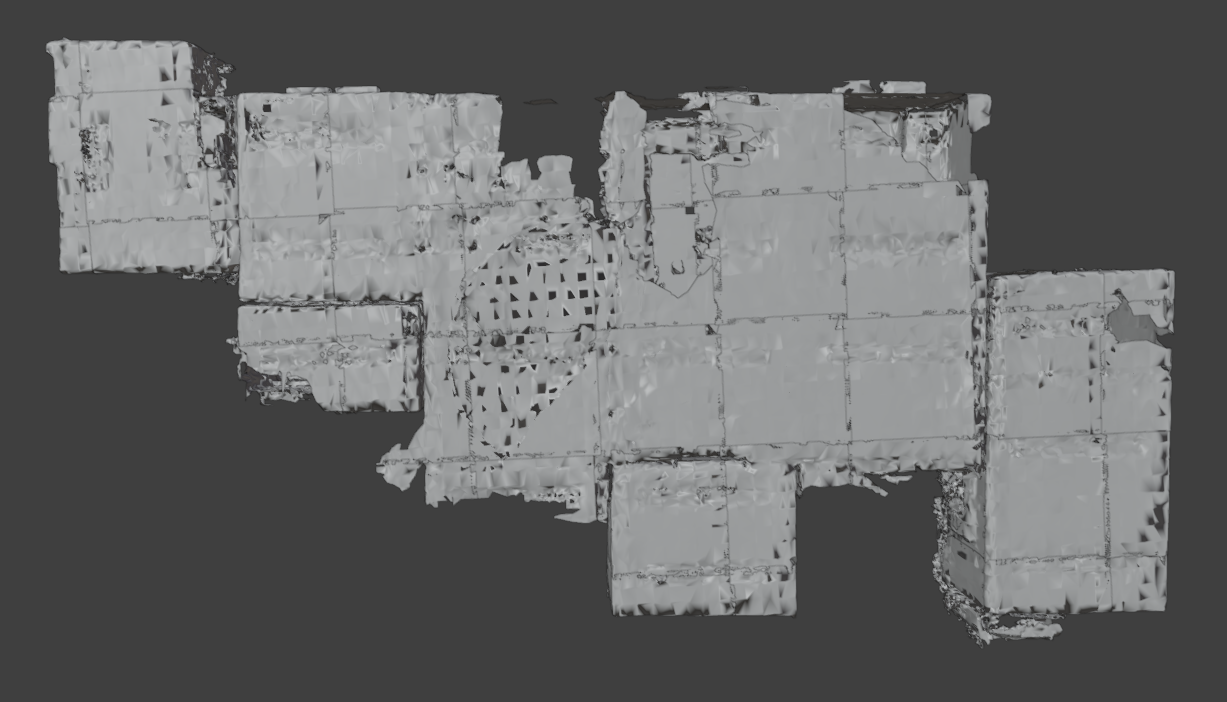
\includegraphics[width=0.7\linewidth]{images/develop_3DModelLabTopView.png}
        \caption{Κάτοψη του εργαστηρίου}
    \end{subfigure}%
    \\
    \begin{subfigure}{1\textwidth}
        \centering
        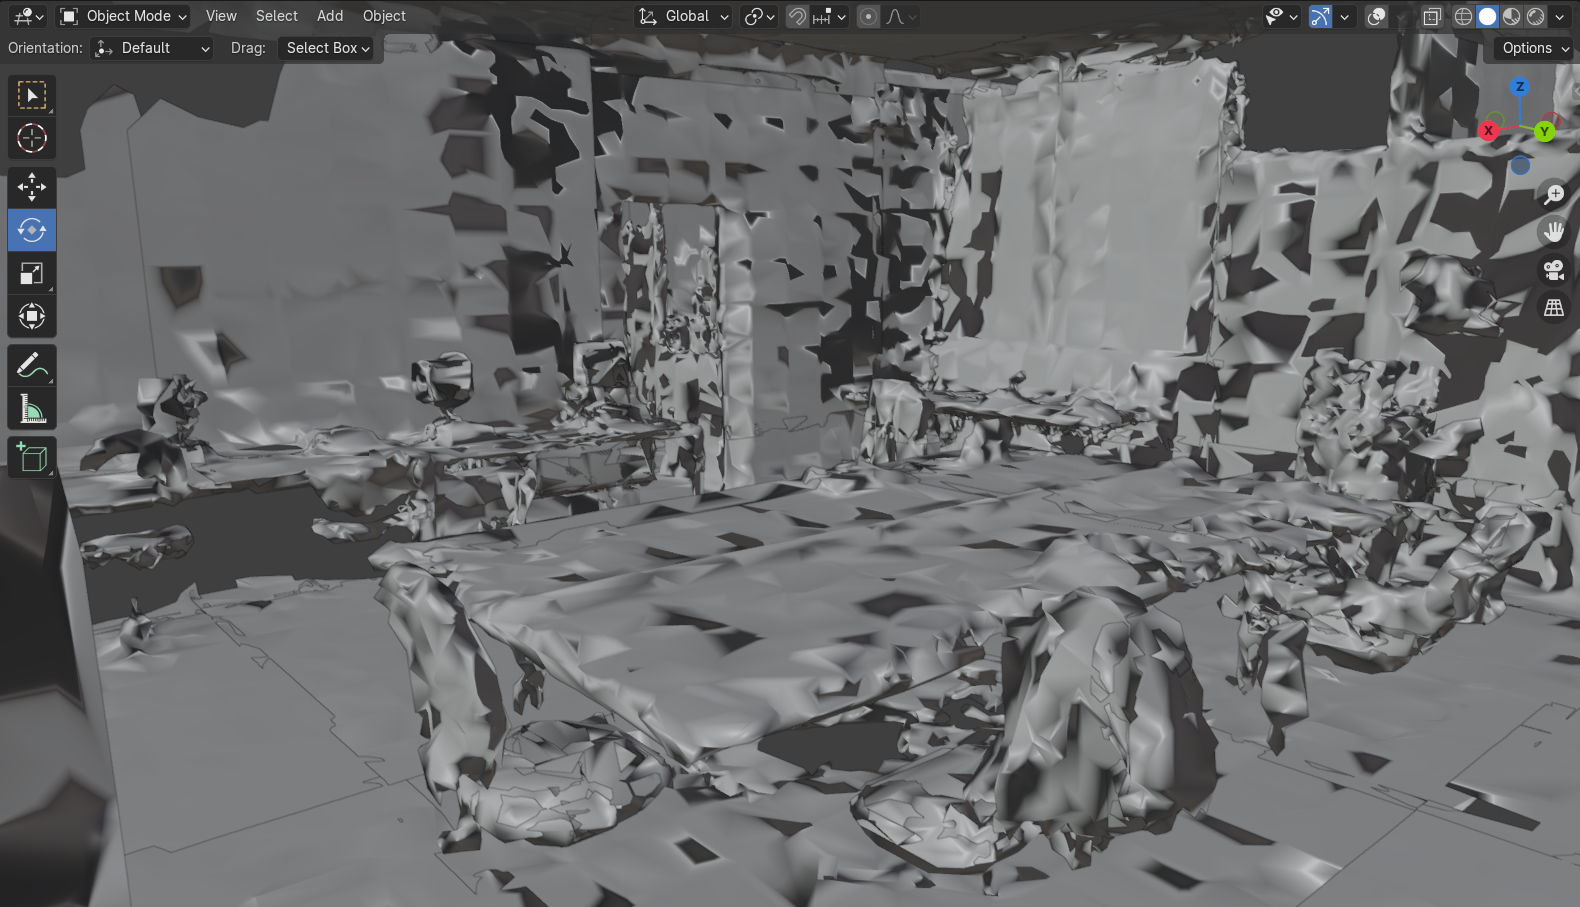
\includegraphics[width=0.7\linewidth]{images/develop_3DModelLabInsideView.png}
        \caption{Εσωτερική απεικόνιση του κύριου χώρου του εργαστηρίου}
    \end{subfigure}%
    \caption{Απεικόνιση του εργαστηρίου με 3D μοντέλο}\label{fig:developModelLab}
\end{figure}

Τέλος, δημιουργήθηκε ο handler \textbf{meshHandler}, στον οποίο προσθέσαμε το Component \hyperref[lst:hideMesh]{\textbf{\textit{hideMesh.cs}}} (\textit{Assets/Scripts}), όπου μπορούμε με χρήση φωνητικών εντολών να κρύψουμε ή να εμφανίσουμε το mesh.

Αφού ολοκληρώσαμε τη διαδικασία χωρικής χαρτογράφησης του χώρου (\hyperref[fig:developSpatialMappingLab]{\schema~\ref*{fig:developSpatialMappingLab}}), πρέπει να υλοποιήσουμε τη λογική για την ανίχνευση των εμποδίων με βάση το mesh που διαθέτουμε. Θα αξιοποιήσουμε την κλάση \code{Physics} του Physics module της Unity, το οποίο χρηισμοποιείται για την εφαρμογή φυσικής σε 3D αντικείμενα. Η κλάση αυτή διαθέτει ποικίλες μεθόδους, οι οποίες μας επιτρέπουν να ανιχνεύσουν τη σύγκρουση δύο αντικείμενων~\cite{unitytechnologies_physics}. Συγκεκριμένα, θα προσπαθήσουμε να εντοπίσουμε το σημείο τομής μιας ακτίνας (ray), που θα αποστέλλουμε από τη θέση του χρήστη, με κάποιο σημείο του mesh.

\begin{figure}[!h]
    \centering
    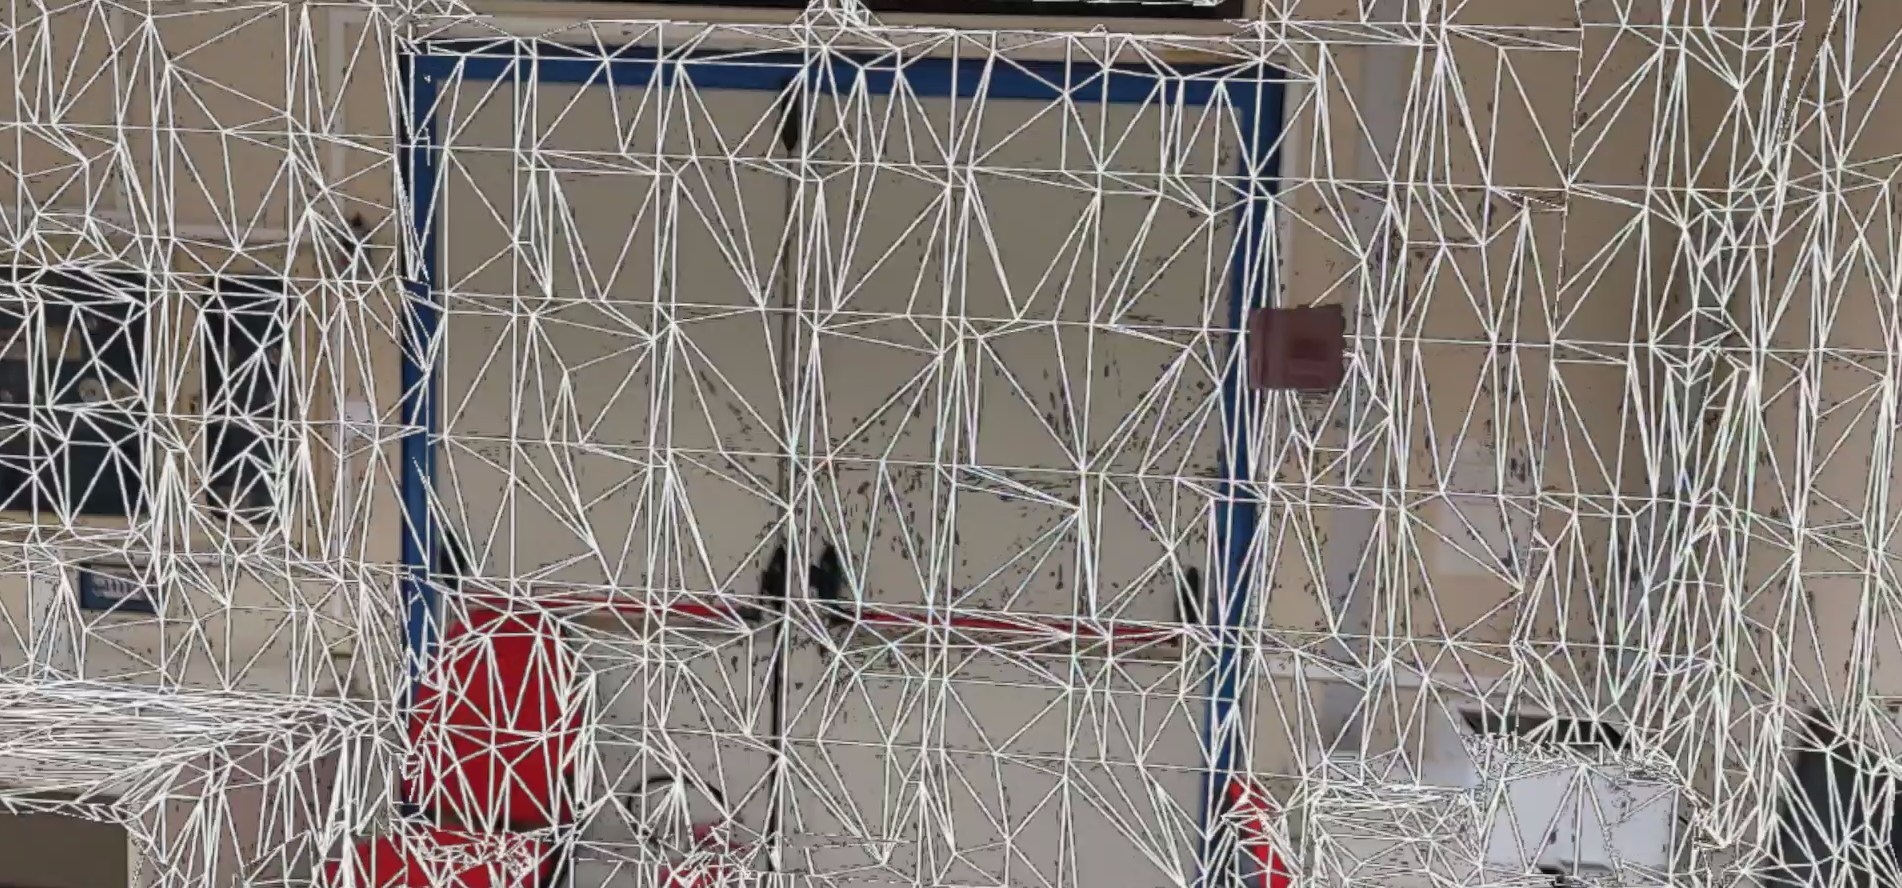
\includegraphics[width=1\textwidth]{images/develop_spatialMappingLab.png}
    \caption{Χωρική χαρτογράφηση του χώρου του εργαστηρίου και απεικόνιση του mesh}\label{fig:developSpatialMappingLab}
\end{figure}

Οι μέθοδοι αυτοί είναι τα \code{RayCast}, \code{BoxCast}, \code{CapsuleCast}, \code{SphereCast}, των οποίων η διαφορά τους έγκειται στο σχήμα της ακτίνας, η οποία `εκπέμπεται'. Στα πλαίσια της εφαρμογής μας, χρησιμοποιήθηκαν δύο μέθοδοι, το \code{RayCast}, που χρησμοποιήθηκε στην αρχή του development, και το \code{BoxCast}, που χρησιμοποιείται στην τελική έκδοση της εφαρμογής. Η δεύτερη μέθοδος επιλέχθηκε λόγω του σχήματος της ακτίνας και του μεγέθους, το οποίο μπορούμε να το ορίσουμε έτσι ώστε να καλύπτει μια ικανοποιητική επιφάνεια μπροστά από το χρήστη. Η μέθοδος δέχεται ως παραμέτρους την αρχική θέση από όπου θα εκπεμθεί η ακτίνα, την κλίμακα αυτής, καθώς έχει το σχήμα κύβου, την περιστροφή της, την κατεύθυνση εκπομπής και τη μέγιστη απόσταση, όπου μέχρι αυτή θα γίνεται έλεγχος επαφής της ακτίνας με κάποια επιφάνειας που διαθέτει collider. Οι ίδιες παράμετροι χρειάζεται και η κλήση της μεθόδου \code{RayCast}, με μόνη εξαίρεση ότι δεν είναι απαραίτητη η κλίμακα και η περιστροφή της ακτίνας, αφού αυτή είναι μονοδιάστατη. Τέλος, η μέθοδος επιστρέφει ένα flag σχετικά με το αν υπήρξε επαφή με αντικείμενο και πληροφορίες σχετικά με αυτή τη σύγκρουση. Στην περίπτωση που υπήρξε επαφή με περισσότερα του ενός αντικείμενα, τότε επιστρέφονται πληροφορίες σχετικά με την πρώτη επαφή, καθώς αυτή θα είναι και η πλησιέστερη από το σημείο έναρξης (Origin Point).

Όπως αντιλαμβανόμαστε από τις παραμέτρους που απαιτούνται από τις δύο μεθόδους, πρέπει να όρισουμε ένα σημείο έναρξης, από όπου θα ξεκινήσει η εκπομπή των ακτινών. Ως σημείο έναρξης ορίζουμε τη θέση του χρήστη, η οποία πρέπει να αλλάζει όταν αυτός θα μετακινείται. Η κατεύθυνση, που επιλέχθηκε, είναι αυτή προς την οποία κοιτά ο χρήστης, καθώς, συνήθως, αυτή είναι και η κατεύθυνση προς την οποία κινείται. Δεδομένου των ανωτέρω, τοποθετήσαμε ορισμένα \code{GameObjects} ως children του \code{GameObject} Main Camera, διότι, σε αυτή την περίπτωση, μαζί με τη θέση και την περιστροφή της κάμερας, που ακολουθεί την κίνηση του κεφαλιού, ανανεώνονται και η θέση και η περιστροφή των \code{GameObjects}. Η ονομασία των αντικειμένων αυτών διαθέτει την κατάληξη `RC' και όλα τους ενσωματώνουν δύο components, το \hyperref[lst:initSingleBox]{\textbf{\textit{initSingleBox.cs}}} (\textit{Assets/Scripts/initiators}) και το \hyperref[lst:singleRaycast]{\textbf{\textit{singleRaycast.cs}}} (\textit{Assets/Scripts}). Το πλήθος των origin points, επομένως και των ακτινών, το μέγεθος και η διάταξη αυτών μπορεί να παραμετροποιηθεί από τις public μεταβλητές του \textbf{variableAggObject} (\hyperref[lst:developVariableAggObjectBoxesPosition]{Κώδικας~\ref*{lst:developVariableAggObjectBoxesPosition}}), ενώ η διαδικασία τοποθέτησης και διαμόρφωσης των διαστάσεων πραγματοποιείται από τη συνάρτηση \code{positionAndScaleBoxes} (\hyperref[lst:developPositionAndScaleBoxes]{Κώδικας~\ref*{lst:developPositionAndScaleBoxes}}), η οποία καλείται κατά την εκτέλεση της εφαρμογής και ανήκει στο component \hyperref[lst:initBoxes]{\textbf{Init Boxes}} (\textit{Assets/Scripts/initiators}), το οποίο και ενσωματώνεται στο \code{GameObject} \textbf{RaycastAndAlertBoxesHandler}. Έπειτα από δοκιμές, επιλέχθηκε η χρήση πέντε σημείων έναρξης εκπομπής ακτινών, τοποθετημένα κάθετα, με τέτοιο τρόπο και διαστάσεις, όπου το πρώτο origin point βρίσκεται στο ύψος των ματιών του χρήστη και το τελευταίο σε ύψος λίγο χαμηλότερο του γονάτου.
\lstinputlisting[style=sharpframe, linerange={7-13,55-59}, label={lst:developVariableAggObjectBoxesPosition}, caption={Μεταβλητές για τη διάταξη των origin points και το μέγεθος των ακτινών}, captionpos=b]{../Unity Project/Thesis-project-2/Assets/Scripts/variablesAggregator.cs}%chktex-file 8
\lstinputlisting[style=sharpframe, linerange={53-89}, label={lst:developPositionAndScaleBoxes}, caption={Η συνάρτηση \textbf{positionAndScaleBoxes} για την τοποθέτηση και αλλαγή διαστάσεων αντικειμένων}, captionpos=b]{../Unity Project/Thesis-project-2/Assets/Scripts/initiators/initBoxes.cs}

Σχετικά με τα components, το \textbf{Init Single Box} διαθέτει ορισμένες public μεταβλητές που αφορόυν κάθε αντικείμενο και χρησιμοποιούνται αποκλειστικά από άλλα components. Αντιθέτως, το script \textbf{Single Raycast} περιέχει τη συνάρτηση, η οποία ξεκινά την εκπομπή της ακτίνας και επιστρέφει τις πληροφορίες για το σημείο επαφής αυτής με το mesh (\hyperref[lst:functionSingleRaycastFunc]{Κώδικας~ζ \ref*{lst:functionSingleRaycastFunc}}). Είναι δυνατό επίσης να επιλέξουμε αν θα γίνει χρήση της μεθόδου \code{RayCast} ή \code{BoxCast} θέτοντας την αντίστοιχη τιμή στη μεταβλητή \code{castType} του \textbf{variableAggObject}.

\lstinputlisting[style=sharpframe, firstline=20, lastline=46, label={lst:functionSingleRaycastFunc}, caption={Η συνάρτηση \textbf{SingleRaycastFunc} για τον εντοπισμό εμποδίων}, captionpos=b]{../Unity Project/Thesis-project-2/Assets/Scripts/singleRaycast.cs}

Επομένως, από πέντε σημεία έναρξης, των οποίων η θέση και η περιστροφή επηρεάζεται από την κίνηση του κεφαλιού του χρήστη, εκπέμπονται ισάριθμες ακτίνες σε σχήμα κύβου (μέθοδος \code{BoxCast}). Αν οι ακτίνες αυτές έρθουν σε επαφή με κάποιο σημείο του πλέγματος, το οποίο ισοδυναμεί με την ύπαρξη εμποδίου προς την κατεύθυνση κίνησης του χρήστη, τότε καταγράφουμε τις πληροφορίες για το σημείο επαφής. Για παράδειγμα, στο \hyperref[fig:developBoxCastExample]{\schema~\ref*{fig:developBoxCastExample}}, μπορούμε να παρατηρήσουμε πέντε κύβους, των οποίων τα κέντρα αποτελούν τα σημεία έναρξης. Οι ακτίνες εκπέμπονται από τα κέντρα και οι πορείες τους αναπαρίστανται με κόκκινες γραμμές, οι οποίες καταλήγουν σε έναν κύβο με κόκκινες ακμές σε περίπτωση που υπήρξε επαφή με το πλέγμα της χωρικής χαρτογράφησης.

\begin{figure}[!ht]
    \centering
    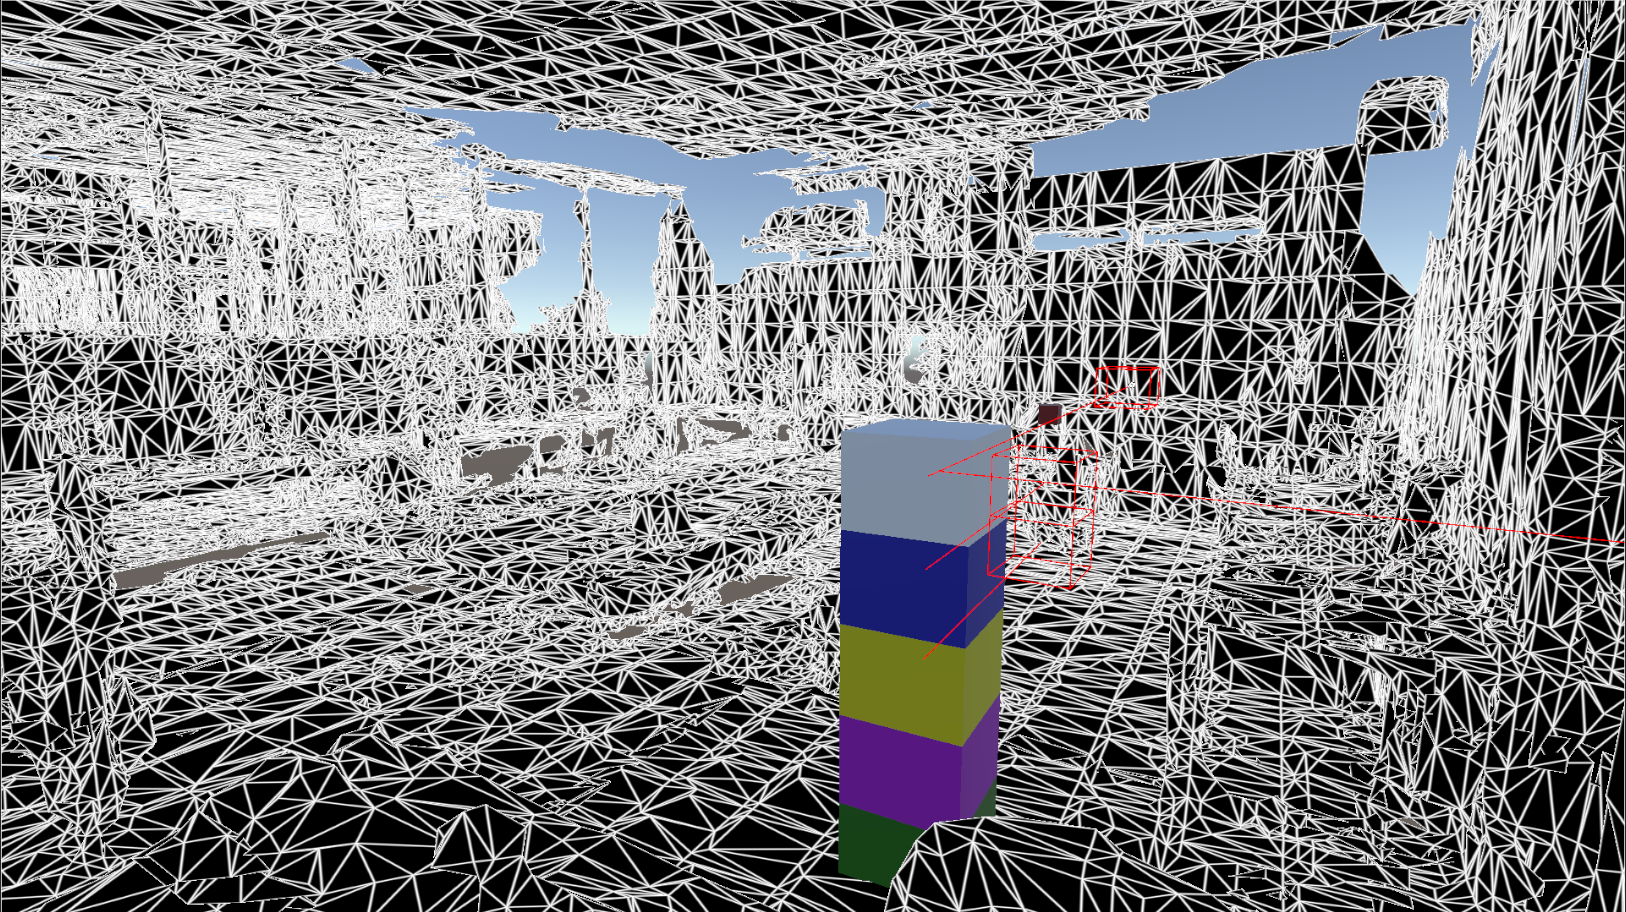
\includegraphics[width=0.8\textwidth]{images/develop_boxCastExample.png}
    \caption{Παράδειγμα εντοπισμού εμποδίων με τη μέθοδο \code{BoxCast}}\label{fig:developBoxCastExample}
\end{figure}

Tα τελευταία ερωτήματα, τα οποία καλούμαστε να απαντήσουμε, με σκοπό να ολοκληρώσουμε τη λειτουργία εντοπισμού εμποδίων αφορούν τη συχνότητα κλήσης της συνάρτησης \textbf{SingleRaycastFunc} και τον τρόπο διαχείρισης πολλαπλών σημείων επαφής. Για τα ερωτήματα αυτά, αναπτύχθηκαν τρεις λύσεις, κάθε μία από τις οποίες έχει τα πλεονεκτήματα και τα μειονεκτήματά της. Κάθε λύση αναπτύχθηκε σε ξεχωριστό component και όλα προστέθηκαν στο \code{GameObject} \textbf{RaycastAndAlertBoxesHandler}

Η πρώτη, χρονικά, λύση, που αναπτύχθηκε, ονομάστηκε \textbf{Scan Mode}. Η εκπομπή των ακτινών ενεργοποιείται `χειροκίνητα', δηλαδή κάθε φορά που ο χρήστης χρησιμοποιεί μια συγκεκριμένη φωνητική εντολή. Τότε, από όλα τα origin points εκπέμπονται τα rays (με μέθοδο \code{BoxCast}). Συγκεντρώνονται σε ένα \code{List} όλα τα σημεία επαφής και επιλέγεται το πλησιέστερο (με χρήση της συνάρτησης \code{findClosestHitPointIndex} του component \textbf{Init Boxes}). Η λογική αυτή περιλαμβάνεται στο component \hyperref[lst:scanCast]{\textbf{Scan Cast}} (\textit{Assets/Scripts/castModes}). Με αυτή τη λύση, ο χρήστης μπορεί να διαχειριστεί τη συχνότητα λήψης ειδοποιήσεων για εμπόδια και να τις λαμβάνει, οπότε αυτός κρίνει απαραίτητο. Ωστόσο, αυτός ο τρόπος ενεργοποίησης μπορεί να αποδειχθεί κουραστικός, ενώ, σε περίπτωση αλλαγής του περιβάλλοντα χώρου, μπορεί να είναι και εσφαλμένος.

Η δεύτερη λύση είναι η \textbf{Continuous Mode} και το component της είναι το \hyperref[lst:continuousCast]{\textbf{Continuous Cast}} (\textit{Assets/Scripts/castModes}). Η λογική σχετικά με την εκπομπή των rays και διαχείριση των πολλαπλών σημείων επαφής είναι με αυτή της προηγούμενης λύσης. Ωστόσο, στην περίπτωση αυτή, ο εντοπισμός εμποδίων πραγματοποιείται σε κάθε frame. Έτσι, ο χρήστης παραμένει πάντα ενήμερος για πιθανά εμπόδια στο χώρο του, ακόμη και πραγματοποιηθεί κάποια αλλαγή σε αυτόν.

Τέλος, η τρίτη λύση αποτελεί και την πιο ιδιάζουσα. Υλοποιείται εντός του component \hyperref[lst:handRaycast]{\textbf{Hand Raycast}} (\textit{Assets/Scripts/initiators}) και ονομάζεται \textbf{Hands Mode}, διότι το σημείο έναρξης των rays αποτελούν το χέρι του χρήστη. Ειδικότερα, εκμεταλλευόμενοι το γεγονός ότι τα χέρια του χρήστη είναι Pointers~\cite{keveleigh_2022_pointers}, που τους επιτρέπουν να αλληλεπιδρούν με εικονικά αντικείμενα σε κοντινή ή μακρινή απόσταση. Στη περίπτωση της αλληλεπίδρασης από μακρινή απόσταση, ο τρόπος εντοπισμού των εικονικών αντικειμένων είναι παρόμοιος με αυτόν που περιγράφηκε στις προηγούμενες λύσεις. Με σημείο έναρξης το χέρι, εκπέμπεται ένα \code{RayCast}, το οποίο αναζητά σημείο επαφής με άλλα εικονικά αντικείμενα, ώστε να αλληλεπιδράση με αυτά. Επομένως, στο αντικείμενο Pointer αποθήκευονται πληροφορίες για το σημείο επαφής, όπως είναι η απόσταση από το χέρι και οι συντεταγμένες του στο χώρο. Επίσης, πρέπει να τονίσουμε ότι τα αντικείμενα Pointers δημιουργούνται και διατηρούνται κάθε φορά που τα χεριά του χρήστη βρίσκονται εντός του πεδίου ορατότητας (FOV) του headset. Με βάση τα ανωτέρω, κάθε φορά που τα χέρια του χρήστη βρίσκονται εντός του FOV, μπορούμε να αναζητήσουμε το σημείο επαφής των raycasts που εκπέμπονται από τα χεριά με το mesh που έχει δημιουργηθεί από τη χωρική χαρτογράφηση και, αν το σημείο αυτό βρίσκεται εντός μια συγκεκριμένης απόστασης, να ειδοποιήσουμε το χρήστη για εμπόδιο (\hyperref[fig:developHandsModeExample]{\schema~\ref*{fig:developHandsModeExample}}).
%(\hyperref[lst:developHandRaycastDetect]{Κώδικας~\ref*{lst:developHandRaycastDetect}}).
Ουσιαστικά, τα raycasts λειτουργούν σαν ένα εικονικό μπαστούνι, το οποίο επιστρέφει feedback στο χειριστή του, όταν `έρθει σε επαφή' με εικονικά αντικείμενα, δηλαδή το mesh.

\begin{figure}[!h]
    \centering
    \begin{subfigure}{1\textwidth}
        \centering
        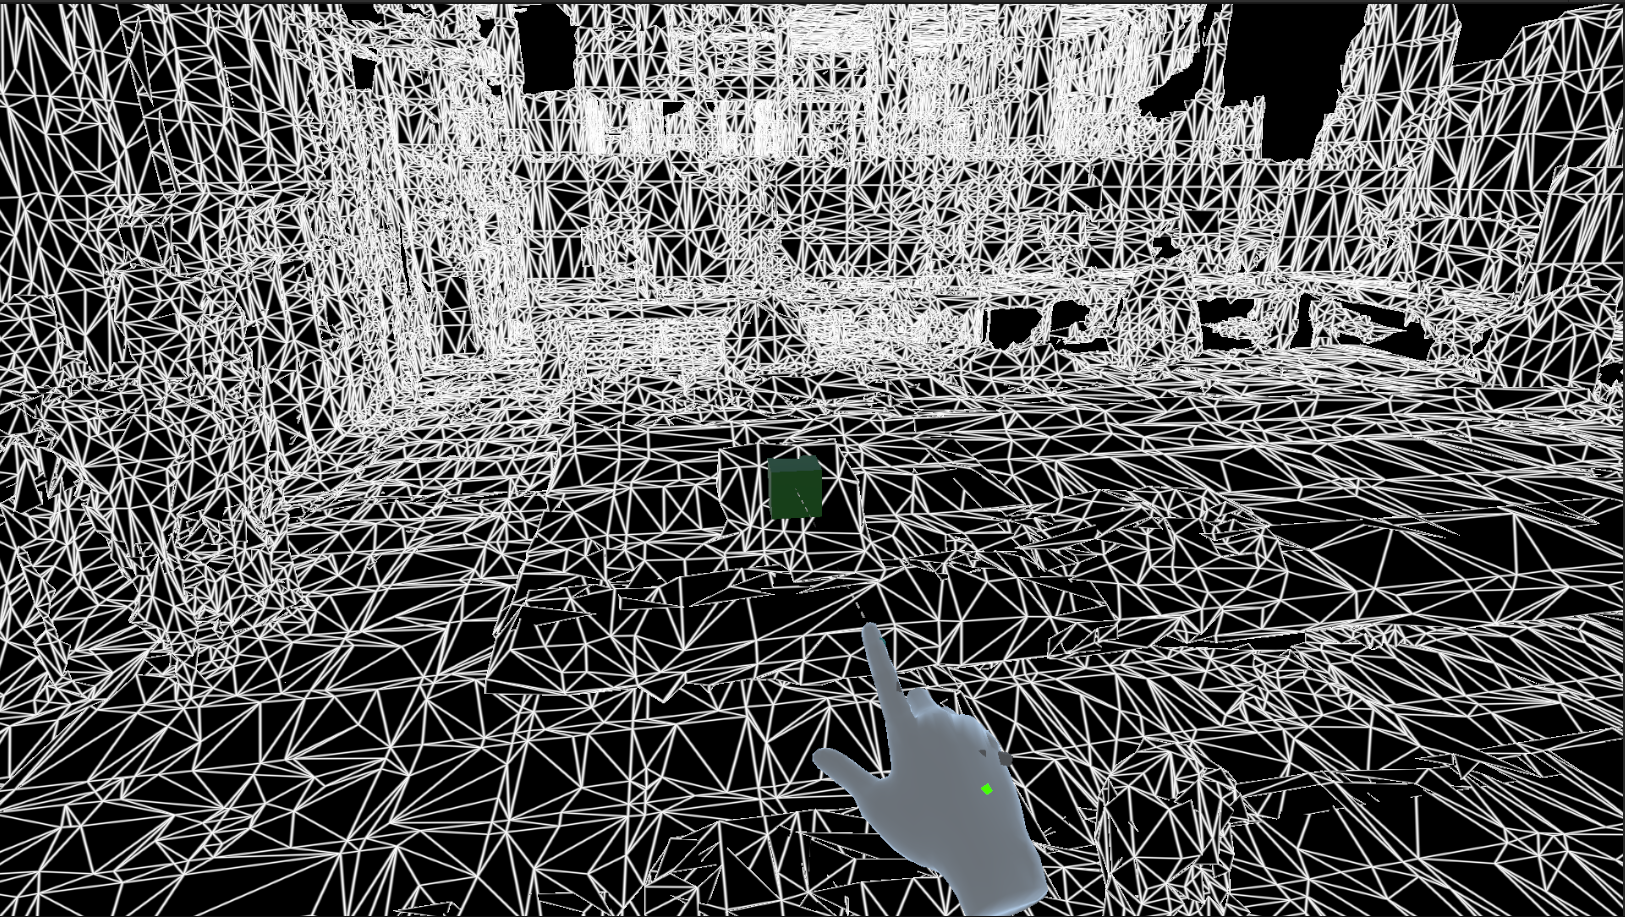
\includegraphics[width=0.7\linewidth]{images/develop_HandsModeSimulationTest.png}
        \caption{}
    \end{subfigure}%
    \\
    \begin{subfigure}{1\textwidth}
        \centering
        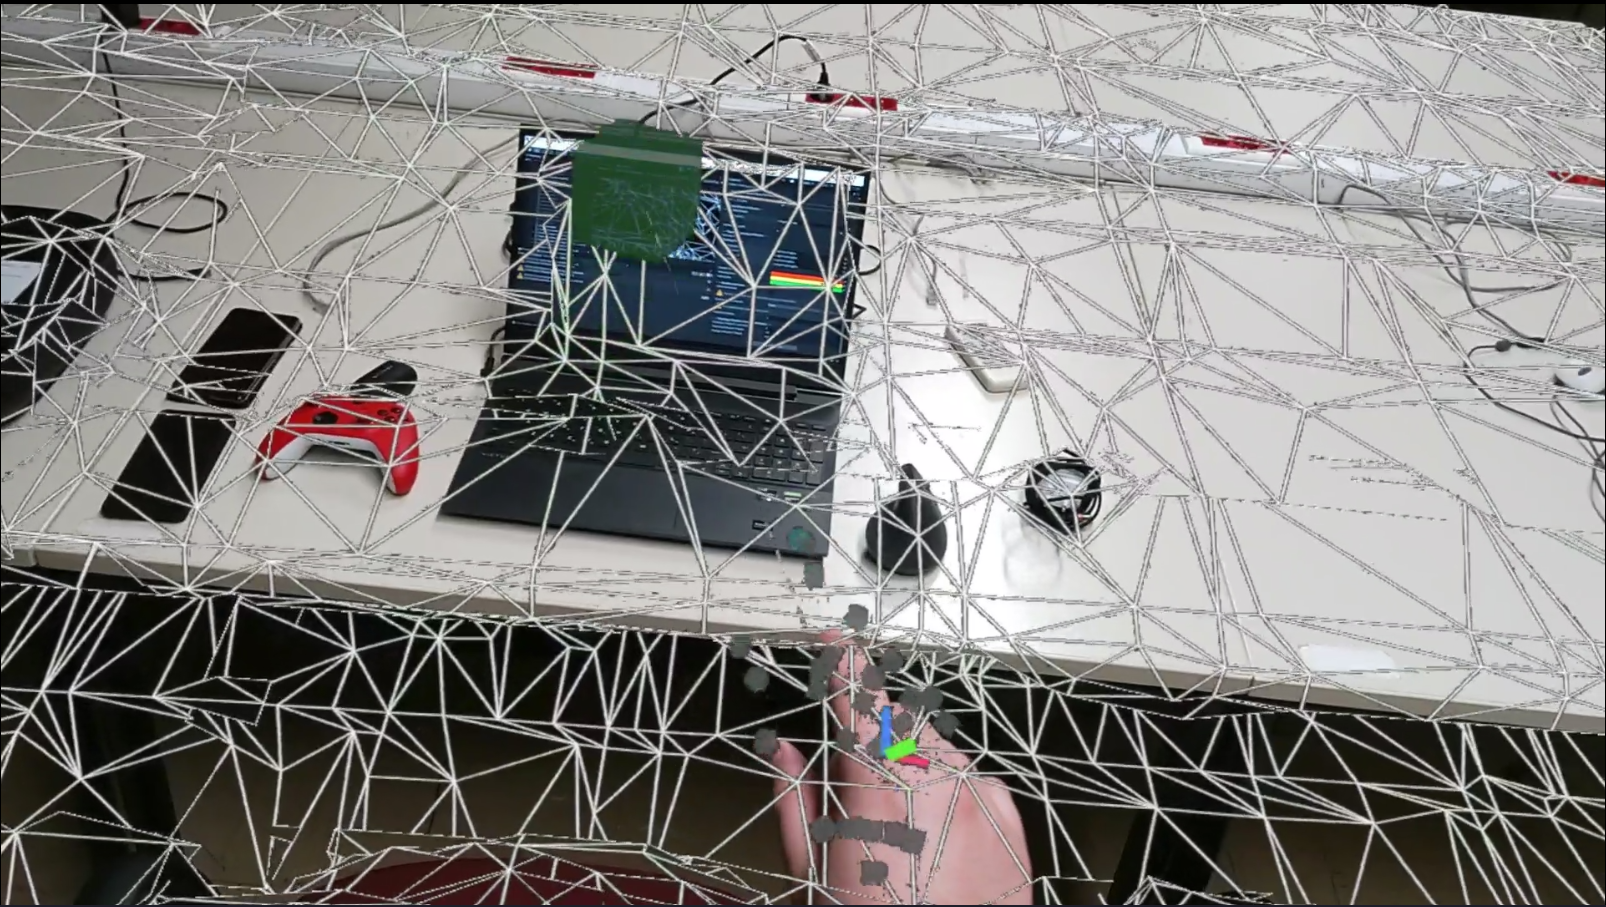
\includegraphics[width=0.7\linewidth]{images/develop_HandsModeLabTest.png}
        \caption{}
    \end{subfigure}%
    \caption{Εντοπισμός εμποδίων με τη λειτουργία \textbf{Hands Mode}}\label{fig:developHandsModeExample}
\end{figure}

% \lstinputlisting[style=sharpframe, linerange={37-71,95-96}, label={lst:developHandRaycastDetect}, caption={Τμήμα της συνάρτησης \textbf{Update} με τη λογική για την εύρεση του σημείου επαφής του Pointer με το mesh}, captionpos=b]{../Unity Project/Thesis-project-2/Assets/Scripts/castModes/handRaycast.cs}

\subsection{Προειδοποίηση Χρήστη}\label{subsec:developWarning}
Μετά τον εντοπισμό εμποδίων, εξίσου ουσιαστική είναι και η έγκαιρη προειδοποίηση του χρήστη για την ύπαρξη αυτών στη διαδρομή του. Σημαντικό ρόλο στην ανάπτυξη αυτής της λειτουργίας θα παίξει η τεχνολογία χωρικού ήχου (spatial sound), που διαθέτει το headset. Η συγκεκριμένη λειτουργία επιτρέπει τη δημιουργία ενός 3D ήχου, ο οποίος θα βοήθησει το χρήστη να αντιληφθεί τη θέση του στο χώρο και ως προς αυτόν.

Αρχικά, θα πρέπει να τοποθετήσουμε την πηγή ήχου στο σημείο που βρίσκεται το εμπόδιο, έτσι ώστε να μπορέσει ο χρήστης να αντιληφθεί που βρίσκεται αυτό. Βασιζόμενοι στη λογική που αναπτύχθηκε και περιγράφηκε στο \hyperref[subsec:developObstacleDetection]{Κεφάλαιο~\ref*{subsec:developObstacleDetection}}, γνωρίζουμε ήδη τη θέση του πλησιέστερου προς το χρήστη σημίου επαφής με το πλέγμα σημείων, το οποίο αντιπροσωπεύει το εμπόδιο. Επομένως, τοποθετούμε στις συντεταγμένες του σημείου αυτού ένα \code{GameObject}, στο οποίο προσθέτουμε το component \textbf{Audio Source}. Με το συγκεκριμένο component, μπορούμε να προσθέσουμε ένα αρχείο, ώστε, από το σημείο όπου τοποθετήσαμε το \code{GameObject} και το οποίο ονομάσαμε \textbf{CommonAlertBox}, να αναπαράγεται ένας προειδοποιητικός ήχος.

\begin{figure}[!h]
    \centering
    \begin{subfigure}{0.5\textwidth}
        \centering
        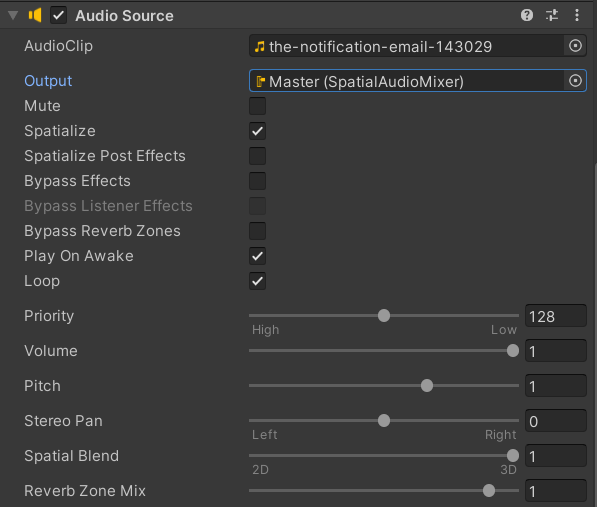
\includegraphics[width=1\linewidth]{images/develop_AudioSourceOne.png}
        \caption{}
    \end{subfigure}%
    \begin{subfigure}{0.5\textwidth}
        \centering
        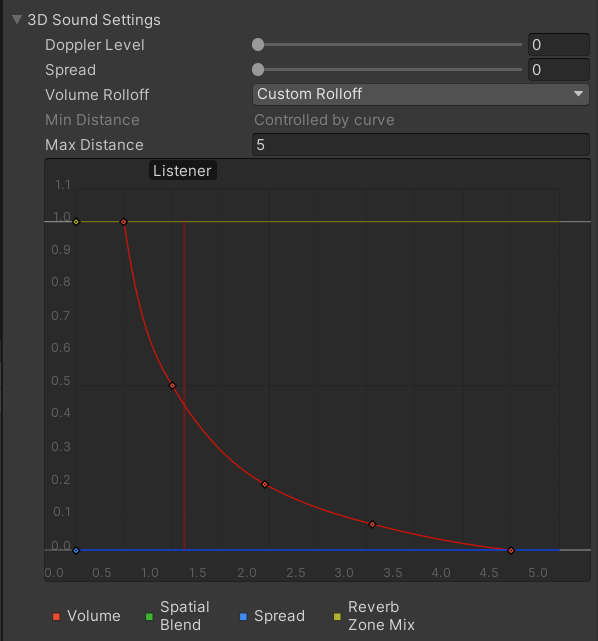
\includegraphics[width=0.8\linewidth]{images/develop_AudioSourceTwo.png}
        \caption{}
    \end{subfigure}%
    \caption{Το component \textbf{Audio Source}}\label{fig:developAudioSource}
\end{figure}

Για να προσδώσουμε στον ήχο τις ιδιότητες ενός χωρικού ήχου, προσθέτουμε ένα Audio Mixer, στο οποίο έχουμε ενσωματώσει το Microsoft Spatializer Mixer effect. Επίσης, ενεργοποιούμε στο \textbf{Audio Source} το spatialization, θετόντας το flag \textbf{Spatialize} σε \textbf{True}, ενώ, παράλληλα, θέτουμε την τιμή \textbf{1} για τη μεταβλητή \textbf{Spatial Blend}. Ορισμένες ακόμη αλλαγές που πραγματοποιήσαμε στο component είναι να ενεργοποιήσαμε τις λειτουργίες \textbf{Play On Awake} και \textbf{Loop}, ώστε ο ήχος να ενεργοποιηθεί με την έναρξη της εφαρμογής και να μην σταματήσει η αναπαραγώγει μέχρι αυτό να υποδειχθεί από τον κώδικα, αντίστοιχα. Τέλος, διαμορφώσαμε την καμπύλη έντασης του ήχου ως προς την απόσταση του χρήστη από την πηγή, έτσι ώστε ο ήχος να γίνεται αισθητός σε απόσταση 5\footnote{Θεωρούμε ότι η αναλογία απόστασης σε μονάδα του περιβάλλοντος Unity προς μέτρα στον πραγματικό κόσμο είναι κατά προσέγγιση 1:1} από την πηγή, να αυξάνεται εκθετικά και να φθάνει το μέγιστο σε απόσταση 1.

Όσον αφορά την τοποθέτηση της πηγής ήχου και τον έλεγχο αναπαραγωγής αυτού στις διάφορες λειτουργίες εντοπισμού εμποδίων, ισχύουν τα κατώθι:
\begin{itemize}
    \item Στη λειτουργία \textbf{Continuous Mode}, ο εντοπισμός πλησιέστερου εμποδίου πραγματοποιείται σε κάθε ανανέωση του frame. Αν εντοπιστεί κάποιο εμπόδιο, τότε η πηγή τοποθετείται στις συντεταγμένες του σημείου και ξεκινά η αναπαραγωγή του προειδοποιητικού ήχου. Αν σε κάποιο update, βρέθει άλλο εμπόδιο, πλησιέστερο προς το χρήστη, τότε η πηγή του ήχου μετακινείται. Αν δεν εντοπιστεί κάποιο εμπόδιο, η αναπαραγωγή του ήχου σταματά.
    \item Στην περίπτωση του \textbf{Scan Mode}, η πηγή ήχου τοποθετείται στο πλησιέστερο εμπόδιο και παραμένει στο σημείο, ακόμη και αν ο χρήστης έχει μετακινηθεί ή αλλάξει κατεύθυνση. Η πηγή ήχου μετακινείται μόνο αν ο χρήστης ενεργοποιήσει ξανά τη λειτουργία με φωνητική εντολή και εντοπιστεί κάποιο νέο εμπόδιο, ενώ, αν δεν εντοπιστεί, τότε ο ήχος απενεργοποιείται.
    \item Στη λειτουργία \textbf{Hands Mode}, η λογική μετακίνησης πηγής και αναπαραγωγής/παύσης του ήψου είναι ίδια με αυτή της λειτουργίας \textbf{Continuous Mode}. Επιπλέον, ο χρήστης έχει τη δυνατότητα, προσωρινά, να παύσει την αναπαραγωγή του ήχου για όσο διάστημα πραγματοποιεί το Pinch gesture. Τέλος, ο ήχος απαενεργοποιείται και στην περίπτωση που τα χέρια βρεθούν εκτός του field-of-view του headset.
\end{itemize}

Αξίζει να αναφερθούμε στο γεγονός ότι υλοποιήθηκε και η ιδέα χρήσης πολλαπλών πηγών και, πιο συγκεκριμένα, μία πηγή για κάθε ray που θα χρησιμοποιούταν για τον εντοπισμό εμποδίων. Αυτή η τεχνική αξιοποίθηκε στην περίπτωση του \textbf{Scan Mode}, ώστε ο χρήστης να είναι ενήμερος για περισσότερα του ενός εμποδίων και να περιορίσουμε τη συχνότητα χρήσης της φωνητικής εντολής για την ενεργοποίηση της λειουργίας. Ωστόσο, κατά τις δοκιμές, η ταυτόχρονη ενεργοποίηση πολλαπλών πηγών ήχου δυσκόλεψε στη διάκριση της κάθε πηγής ήχου και επομένως της θέσης του εμποδίου, λόγω της ιδιαίτερα κοντινής απόστασης στην οποία τοποθετούνταν.

Τέλος, εκτός από την ηχητική προειδοποίηση του χρήστη, αναπτύχθηκαν δύο ακόμη μέθοδοι: μία οπτική και μία με απτική ανάδραση. Η οπτική προειδοποίηση απευθύνεται σε άτομα που δεν αντιμετωπίζουν πλήρη απώλεια όρασης και μπορούν να αντιληφθούν χρώματα και σχήματα. Σε αυτό τον τρόπο προειδοποίησης, τοποθετούμε τέσσερα σχήματα μπροστά στο οπτικό πεδίο του χρήστη, το καθένα σε μια διαφορετική σχέση: στο πάνω, δεξί, κάτω και αριστερό μέρος του πεδίου του. Όταν εντοπιστεί κάποιο εμπόδιο, ανάλογα με τη θέση του εμποδίου ως προς τη κατεύθυνση που κοιτά ο χρήστης, τα αντίστοιχα σχήματα αρχίζουν να αναβοσβήνουν. Το χρώμα των σχημάτων αλλάζει ανάλογα με την απόσταση του χρήστη από το εμπόδιο. Ξεκινώντας από το πράσινο και όσο πλησιάζει προς το εμπόδιο, το χρώμα αλλάζει σε κίτρινο και τέλος σε κόκκινο. Κάθε σχήμα αποτελεί ένα \code{GameObject}, το οποίο διαθέτει το component \hyperref[lst:flashingLight]{\textbf{Flashing Light}} (\textit{Assets/Scripts}), που περιέχει τη λογική για το flashing effect και τη θέση του αντικειμένου στο πεδίο ορατότητας του χρήστη. Ο κώδικας για την επιλογή ενεργοποίησης των κατάλληλων αντικειμένων ανάλογα με την θέση των εμποδίων είναι στο component \hyperref[lst:initFlashHandler]{\textbf{Init Flash Handler}} (\textit{Assets/Scripts/initiators}) του \textbf{RaycastAndAlertBoxesHandler}.

Τέλος, αναπτύχθηκε και μέθοδος της απτικής ανάδρασης για την προειδοποίηση του χρήστη. Για τη μέθοδο αυτή, χρησιμοποιήθηκε η συσκευή Microsoft XBOX Series controller (\hyperref[fig:xboxController]{\schema~\ref*{fig:xboxController}}). Πρόκειται για ένα χειριστήριο, το οποίο επιλέχθηκε λόγω της απλότητας της ασύρματης σύνδεσης αυτού με τον υπολογιστή, για την ανάπτυξη του κώδικα, και του headset, για την πρακτική χρήση αυτού. 
Επιπλέον, η Unity παρέχει έτοιμες βιβλιοθήκες με κλάσεις, οι οποίες μας επιτρέπουν να αναγνωρίσουμε την σύνδεση/αποσύνδεση του χειριστηρίου, το input του χρήστη μέσω αυτού, καθώς και να ελέγξουμε τμήματα αυτού.
\begin{figure}[!h]
    \centering
    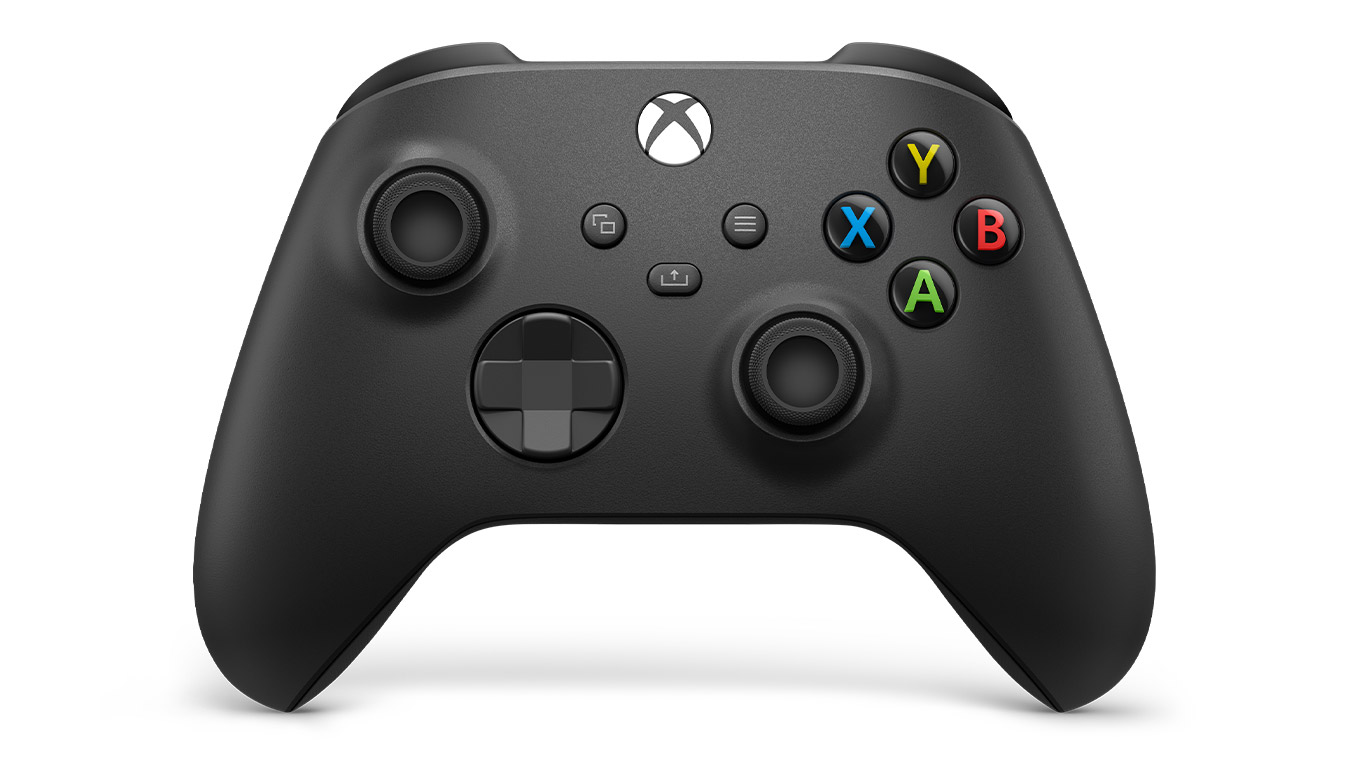
\includegraphics[width=0.6\textwidth]{images/xboxController.jpg}
    \caption{Το χειριστήριο Microsoft XBOX Series {\footnotesize(Πηγή: microsoft.com)}}\label{fig:xboxController}
\end{figure}
Η απτική ανάδραση επιτυγχάνεται με την ενεργοποίηση ενός εκ των δύο μοτέρ που διαθέτει το controller, ένα σε κάθε πλευρά αυτού. Ανάλογα με τη θέση του εμποδίου ως προς την κατεύθυνση που κοιτά ο χρήστης, ενεργοποιείται το αντίστοιχο μοτέρ παράγοντας μια παλμική δόνηση. Όσο πιο πολύ πλησιάζει ο χρήστης στο εμπόδιο, τόσο η ένταση της δόνησης και η συχνότητα των παλμών αυξάνονται. Τέλος, ο χρήστης μπορεί να ενεργοποίηση και να απενεργοποιήση αυτόν τον τρόπο προειδοποίησης πιέζοντας τα κουμπιά `A' και `B' αντίστοιχα. Η διαχείριση του χειριστηρίου πραγματοποιείται από το component \hyperref[lst:initRumbleHandler]{\textbf{Init Rumble Handler}} (\textit{Assets/Scripts/initiators}) του αντικειμένου \textbf{RaycastAndAlertBoxesHandler}.

\subsection{Φωνητικές Εντολές}\label{subsec:developVoiceCommands}
Αφού ολοκληρώσαμε την ανάπτυξη της λογικής για τον εντοπισμό εμποδίων και την προειδοποίηση του χρήστη, καλούμαστε τώρα να δώσουμε στο χρήστη τη δυνατότητα ελέγχου αυτών των λειτουργιών. Αυτό καθίσταται εφικτό με τη χρήση φωνητικών εντολών.

Η δυνατότητα χρήσης φωνητικών εντολών μπορεί να εναργοποιηθεί από το \textbf{MixedRealityToolkit}, στην καρτέλα `Input'. Εκεί μπορούμε να προσθέσουμε τις λέξεις-κλειδιά, εκφρασμένες στην Αγγλική γλώσσα, οι οποίες θα αποτελέσουν τις εντολές της εφαρμογής. Στη συνέχεια δημιουργούμε το \code{GameObject} \textbf{SpeechInputHandler\_Global}, στο οποίο προσθέτουμε το component \textbf{SpeechInputHandler} (\hyperref[fig:developVoiceCommands]{\schema~\ref*{fig:developVoiceCommands}}), το οποίο προσφέρει το MRTK~\cite{speechinputhandler} για τη διαχείριση των φωνητικών εντολών. Συγκεκριμένα, όταν προσθέτουμε μια νέα φωνητική εντολή, επιλέγουμε την λέξη-κλειδί, η οποία θα την ενεργοποιεί, και ένα \code{GameObject}. Το \code{GameObject} διαθέτει components, από τα οποία επιλέγουμε μία συνάρτησή τους, η οποία θα εκτελείται, όταν θα χρησιμοποιείται η εντολή.

\begin{figure}[!h]
    \centering
    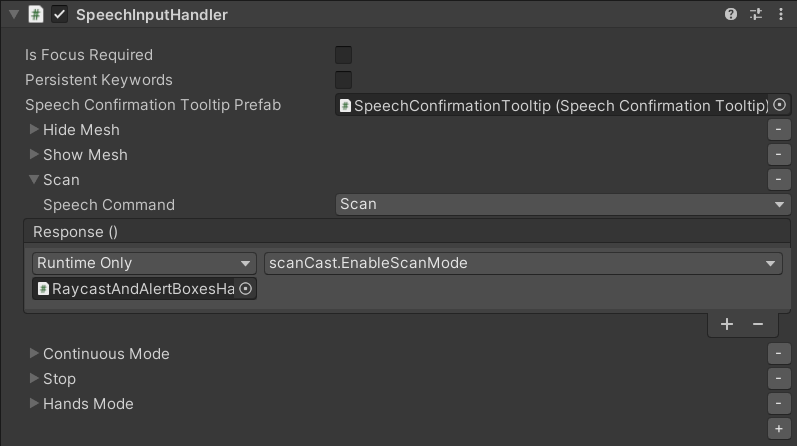
\includegraphics[width=1\textwidth]{images/develop_speechInputHandler.png}
    \caption{Το component \textbf{SpeechInputHandler} και οι φωνητικές εντολές της εφαρμογής}\label{fig:developVoiceCommands}
\end{figure}

Οι διαθέσιμες φωνητικές εντολές, καθώς και οι λειτουργίες τους, είναι οι εξής:
\begin{itemize}
    \item \textbf{Hide Mesh}:
    \begin{itemize}
        \item \textbf{Συνάρτηση}: hideMeshFunc (\textbf{Component}: \hyperref[lst:hideMesh]{\textit{hideMesh.cs}})
        \item \textbf{Λειτουργία}: Απόκρυψη απεικόνισης του mesh
    \end{itemize}
    \item \textbf{Show Mesh}:
    \begin{itemize}
        \item \textbf{Συνάρτηση}: showMeshFunc (\textbf{Component}: \hyperref[lst:hideMesh]{\textit{hideMesh.cs}})
        \item \textbf{Λειτουργία}: Απεικόνιση του mesh
    \end{itemize}
    \item \textbf{Scan}:
    \begin{itemize}
        \item \textbf{Συνάρτηση}: EnableScanMode (\textbf{Component}: \hyperref[lst:scanCast]{\textit{scanCast.cs}})
        \item \textbf{Λειτουργία}: Ενεργοποίηση του \textbf{Scan Mode} για τον εντοπισμό εμποδίων
    \end{itemize}
    \item \textbf{Continuous Mode}:
    \begin{itemize}
        \item \textbf{Συνάρτηση}: continuousModeGlobalToggle (\textbf{Component}: \hyperref[lst:continuousCast]{\textit{continuousCast.cs}})
        \item \textbf{Λειτουργία}: Ενεργοποίηση/απενεργοποίηση του Continuous Mode για τον εντοπισμό εμποδίων
    \end{itemize}
    \item \textbf{Stop}:
    \begin{itemize}
        \item \textbf{Συνάρτηση}: EnableStopMode (\textbf{Component}: \hyperref[lst:stopCast]{\textit{stopCast.cs}})
        \item \textbf{Λειτουργία}: Απενεργοποίηση του \textbf{Continuous Mode} και παύση όλων των προειδοποιητικών ήχων
    \end{itemize}
    \item \textbf{Hands Mode}: 
    \begin{itemize}
        \item \textbf{Συνάρτηση}: enabledHandABToggle (\textbf{Component}: \hyperref[lst:handRaycast]{\textit{handRaycast.cs}})
        \item \textbf{Λειτουργία}: Ενεργοποίηση/απενεργοποίηση της λειτουγρίας \textbf{Hands Mode}
    \end{itemize}
\end{itemize}